\documentclass[../main.tex]{subfiles}

\begin{document}

    The interaction with the environments has to be streamlined and automated to an extent that no manual work is required for deployments to follow the \gls{devops} principles.
    This is achieved with a \gls{gitops} pipeline that is taking care of \acrlong{cd}.

    In a more classical approach, many components might be deployed into test, staging and production environments, which are set up using configuration management tools like \gls{puppet} or \gls{ansible}.
    The service versions in the environments are managed independently and manually and there is no clear representation of the desired state.

    Using a classical approach that requires manual steps can be expensive but might work for predominantly homogeneous environments.
    Once new execution environments are added when migrating to a \gls{hybrid_cloud} setup, the amount of effort it takes will increase drastically.
    Not only will deployment effort increase but also complexity (Fig.~\ref{fig:deploy_process_timeline}).

    \begin{figure}[h]
        \centering
        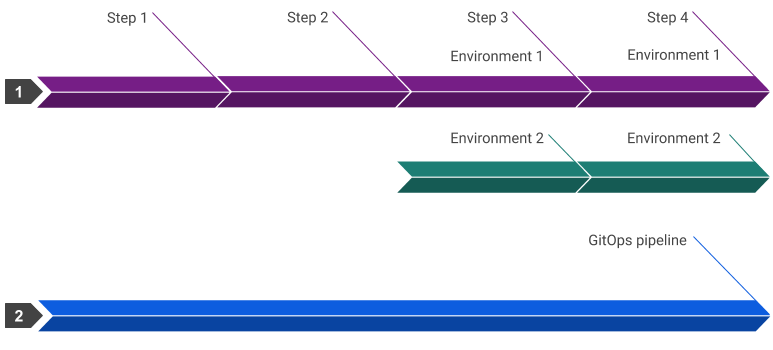
\includegraphics[width=.9\linewidth]{img/concepts_deploy_process_v3.png}
        \captionsetup{justification=centering}
        \caption{
            A classical approach that involves manual steps requiring user interaction, which multiplies in effort when adopting \gls{cloud} (1), versus a streamlined, automated pipeline (2).
        }
        \label{fig:deploy_process_timeline}
    \end{figure}

    \gls{gitops} is an approach for building deployment pipelines that evolved around \gls{git}.
    Everything required to build an environment is stored as code in a \gls{git} repository.
    Storing everything as code enables the use of declarative definitions of the desired state that can be applied to the execution environments automatically and incrementally.
    Once the repository changes, the deployment pipeline is triggered either through a pull- or a push-mechanism.\cite{gitops}

    I am using a \gls{gitops} workflow for my \gls{hybrid_cloud} deployments as it allows me to fully exploit the declarative desired state concept of \gls{kubernetes}.
    The basis of my workflow will be a \gls{git} metadata repository hosting all application manifests.
    Each change will trigger the workflow and update all execution environments.

\end{document}

